\chapter{Выполнения задания}

\section{Реализация алгоритма расчета DF для выборки документов}

В листинге \ref{lst:tf_alg} приведены реализации алгоритма расчета документной частоты DF для каждого терма и следующая за ним сортировка массива DF методом пузырька. В качестве термов в данной реализации рассматриваются слова, состоящие из латинских букв. В качестве документов рассматриваются строки, состоящие из таких слов, пробелов и знаков пунктуации.

\clearpage

\lstinputlisting[label=lst:tf_alg,caption=Функция  реализации алгоритма расчета документной частоты и пузырьковой сортировки массива DF, firstline=11,lastline=38]{main.c}
\clearpage
\section{Графовые представления}

\begin{figure}[h]
	\centering
	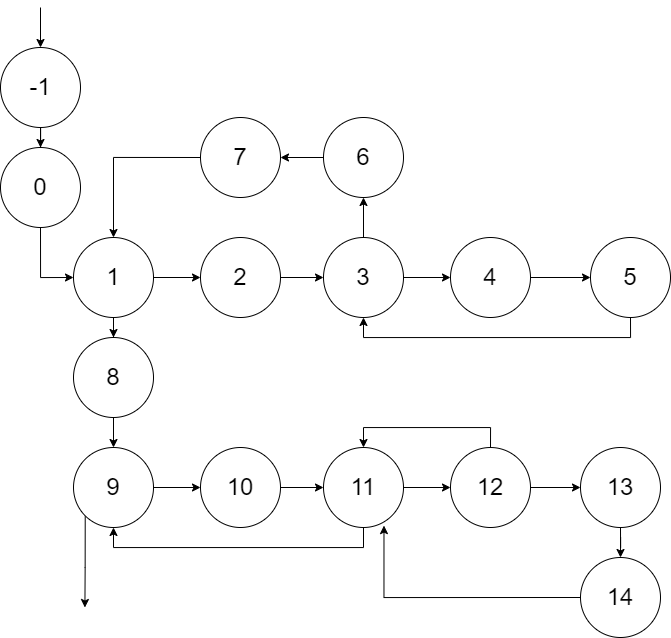
\includegraphics[width=0.9\textwidth]{img/dz-Граф управления.drawio.png}
	\caption{Операционный граф}
	\label{fig:g1}
\end{figure}

\begin{figure}[h]
	\centering
	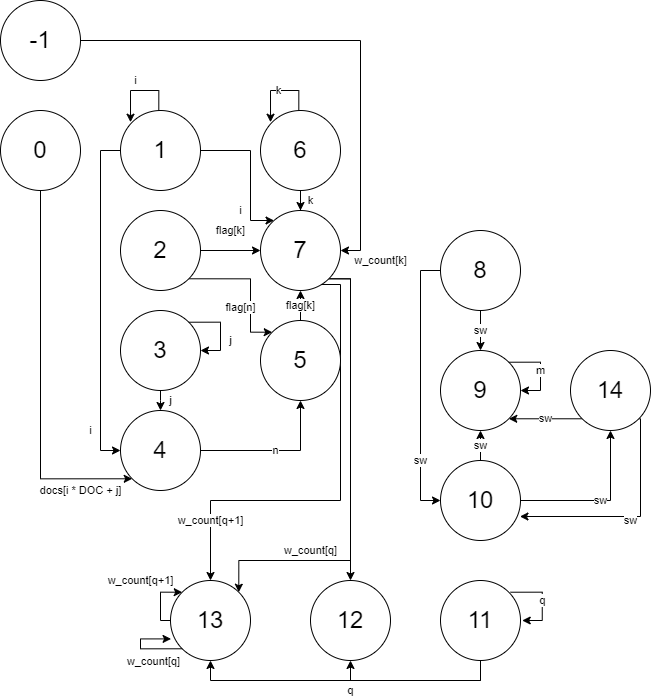
\includegraphics[width=0.9\textwidth]{img/dz-Информационный граф.drawio.png}
	\caption{Информационный граф}
	\label{fig:g2}
\end{figure}

\begin{figure}[h]
	\centering
	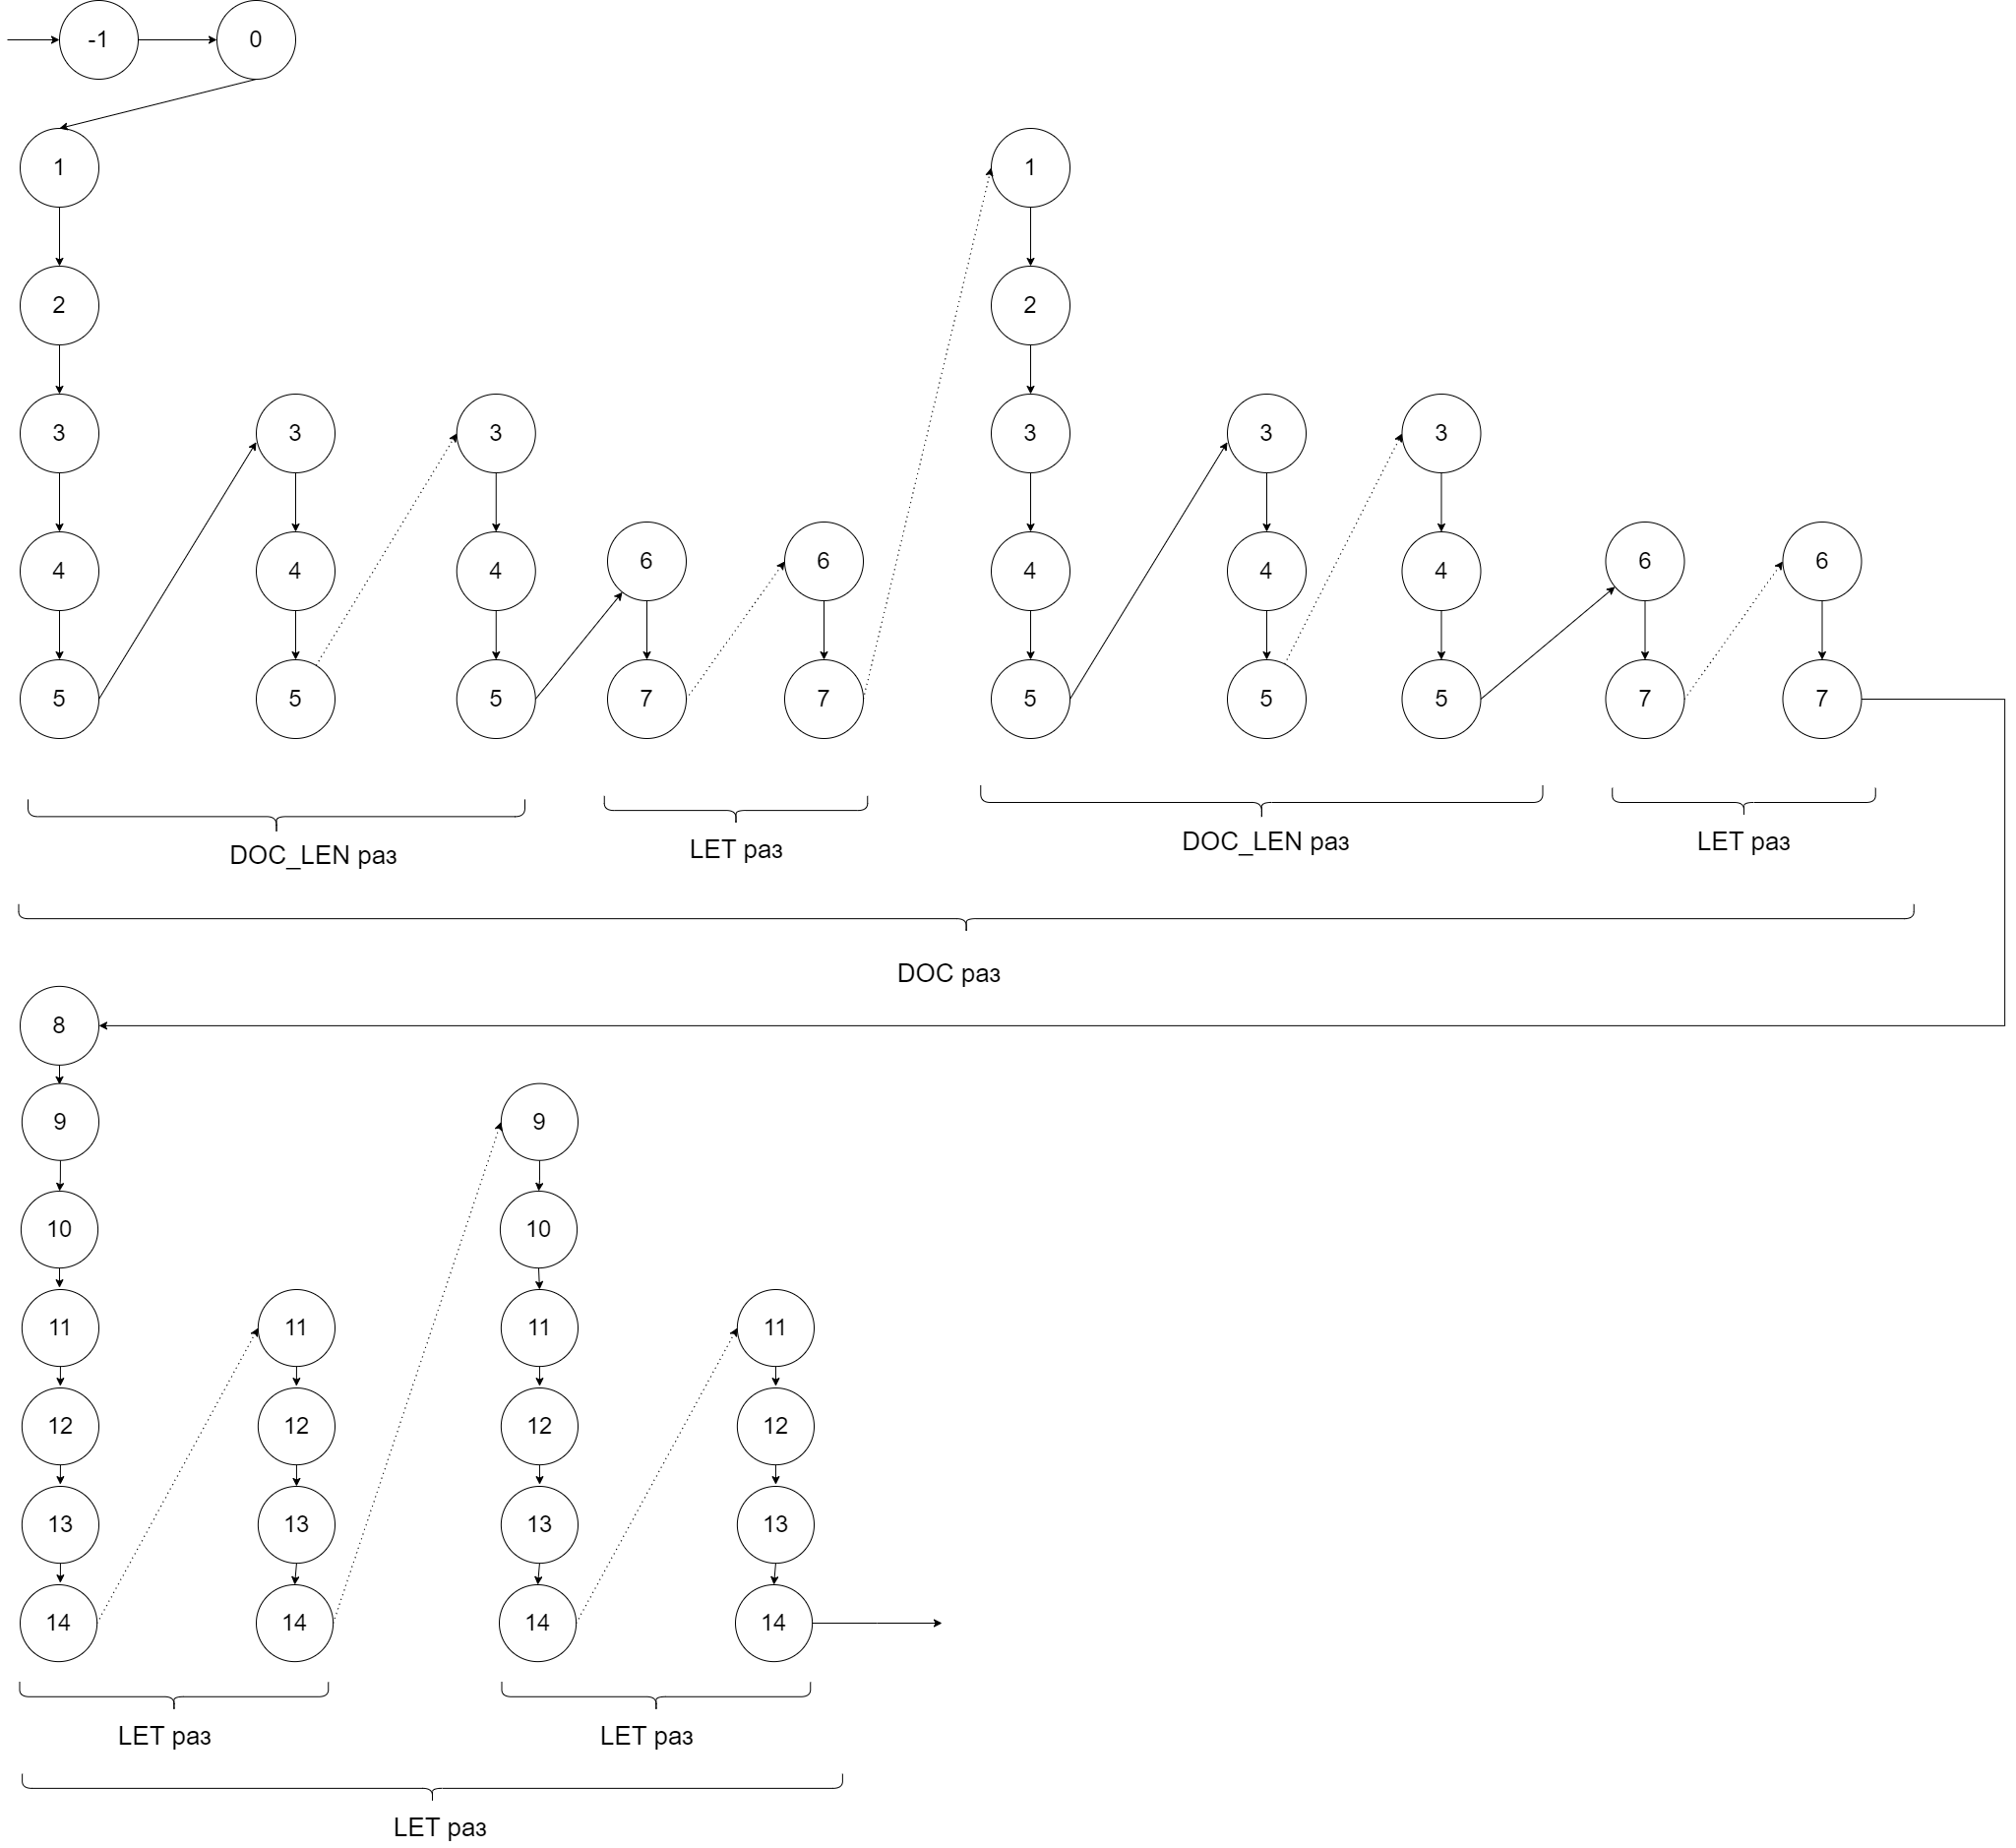
\includegraphics[width=0.9\textwidth]{img/dz-операционная история.drawio.png}
	\caption{Операционная история}
	\label{fig:g3}
\end{figure}

\begin{figure}[h]
	\centering
	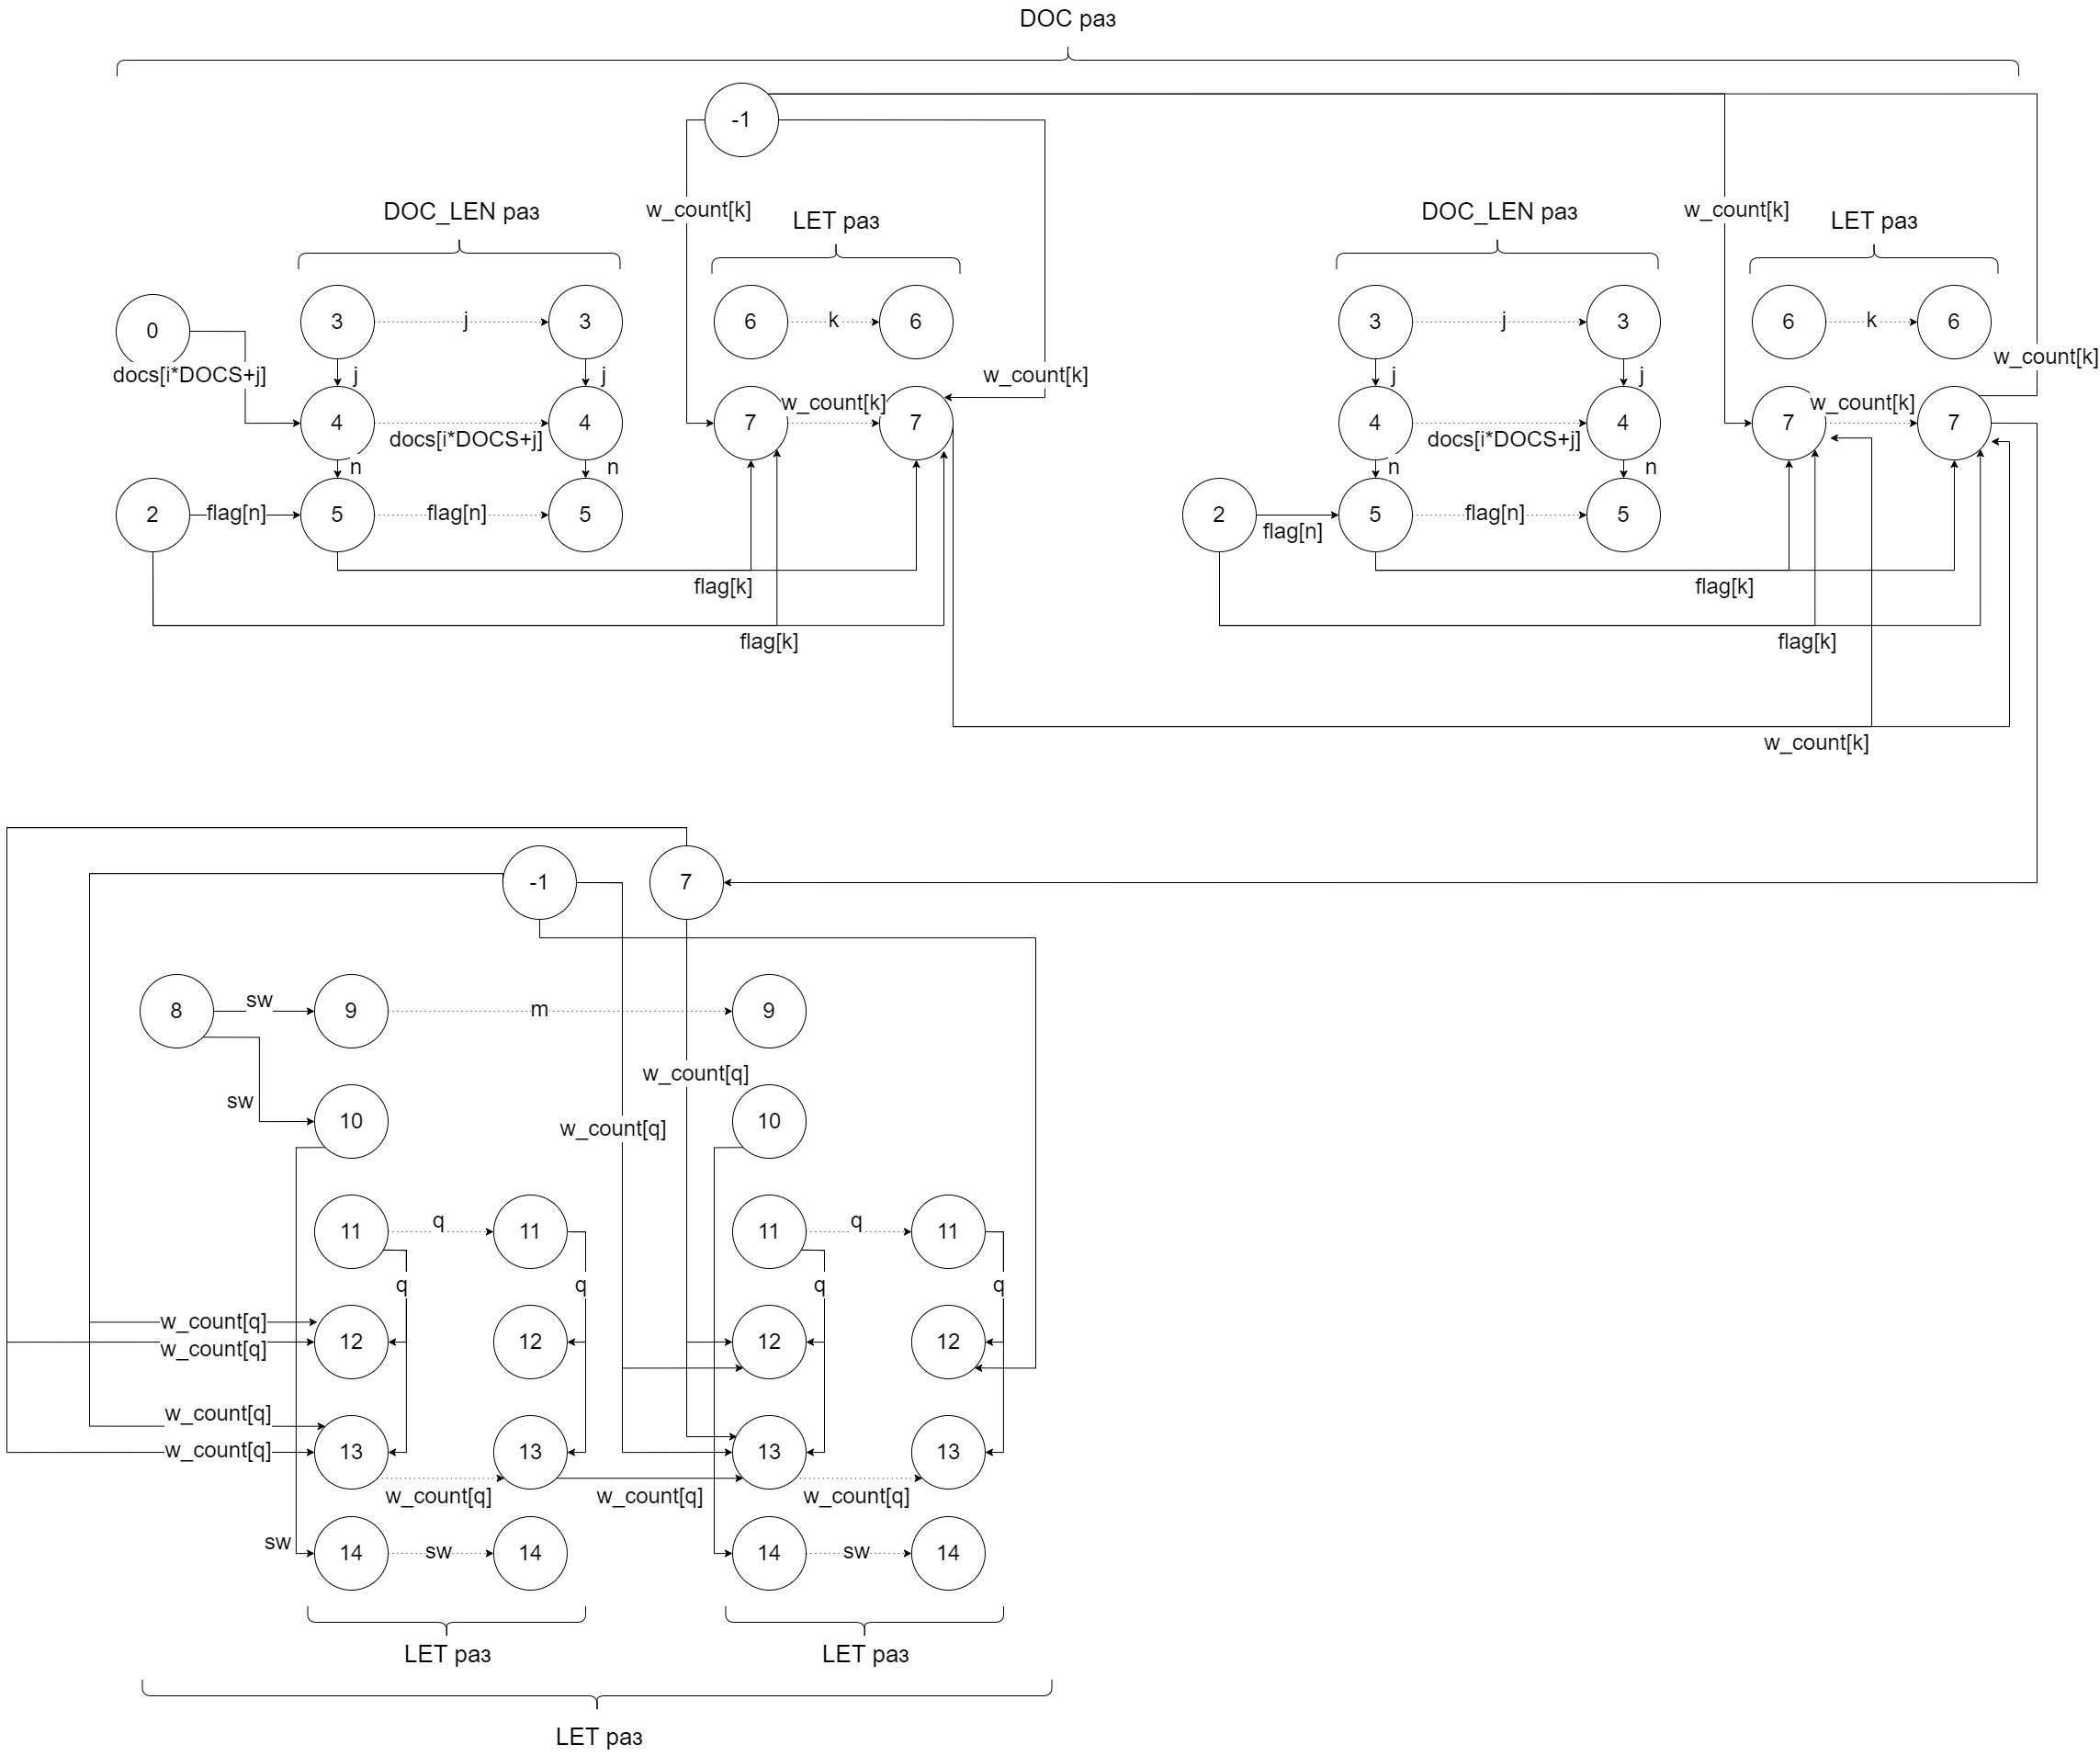
\includegraphics[width=0.9\textwidth]{img/dz-Информационная история.drawio.png}
	\caption{Информационная история}
	\label{fig:g34}
\end{figure}